% !Mode:: "TeX:UTF-8"
% 请注意,此文件的编码方式一定要设置为UTF-8 无DOM模式
% 否则中文显示乱码!
% 可以用notepad++ 或ultraedit查看/更改文件编码方式

\documentclass[a4paper,12pt]{article}

%插入超链接,并且去除超链接的颜色下划线等特性
\usepackage[hidelinks]{hyperref}

%该宏包可以添加伪代码CLRS《算法导论》**第三版**模式
%clrscode3e.sty放在项目根目录下即可
\usepackage{clrscode3e}

%插入数学公式
\usepackage{amsmath}

%中文包
\usepackage{xeCJK}
\setCJKmainfont{SimSun}

%设置页边距
\usepackage[top=0.93in,bottom=0.8in,left=1.1in,right=1in]{geometry}

\usepackage{xcolor}

%为了插入代码
\usepackage{listings}

\definecolor{codegreen}{rgb}{0,0.6,0}
\definecolor{codegray}{rgb}{0.5,0.5,0.5}
\definecolor{codepurple}{rgb}{0.58,0,0.82}
\definecolor{backcolour}{rgb}{0.95,0.95,0.92}

\lstdefinestyle{mystyle}{
    backgroundcolor=\color{backcolour},
    commentstyle=\itshape\color{codegreen},
    keywordstyle=\color{magenta},
    numberstyle=\tiny\color{codegray},
    stringstyle=\color{codepurple},
    basicstyle=\footnotesize,
    breakatwhitespace=false,
    breaklines=true,
    captionpos=b,
    keepspaces=true,
    numbers=left,
    numbersep=5pt,
    showspaces=false,
    showstringspaces=false,
    showtabs=false,
    tabsize=4
}

\lstdefinestyle{default}{
    backgroundcolor=\color{backcolour},
    commentstyle=\itshape,
    numberstyle=\tiny,
    basicstyle=\footnotesize,
    breakatwhitespace=false,
    breaklines=true,
    captionpos=b,
    keepspaces=true,
    numbers=left,
    numbersep=5pt,
    showspaces=false,
    showstringspaces=false,
    showtabs=false,
    tabsize=4
}

\lstset{style=default}

%为了插入图片
%\usepackage{graphicx}

%为了画图
\usepackage{tikz}
\usetikzlibrary{positioning}
\usetikzlibrary{arrows.meta} % L ATEX and plain TEX when using Tik Z
\usetikzlibrary{shapes.geometric}
\usetikzlibrary{calc}

%首段缩进
\usepackage{indentfirst}

%插入表格,自定义表格横竖线
\usepackage{tabularx,hhline}% http://ctan.org/pkg/{tabularx,hhline}

%数学符号,三角形△
\usepackage{amssymb}

\title{Assignment 7\\Algorithm Design and Analysis}

\author{\href{http://bitjoy.net}{bitjoy.net}}
\date{January 16, 2016}

\begin{document}

\maketitle

\section*{1\quad Bin Packing}

以下答案整理自百度文库\footnote{\url{http://wenku.baidu.com/view/f6e7f80590c69ec3d5bb755f.html}}。

假设有$n$个物品$A_1,A_2,...,A_n$,体积分别为$a_1,a_2,...,a_n\in (0,1]$,有若干个容量为1的箱子$B_1,B_2,...$,问怎样把这$n$个物品都装到箱子里,使所用的箱子越少越好。

这里提供两种解法,分别是Next Fit(NF)和First Fit Decreasing(FFD) 算法。

\subsection*{\textnormal{1.1\quad Next Fit(NF)}}

对于每一个物品$A_i$,如果当前箱子$B_j$能装下,则装入当前箱子,否则把当前箱子关闭,新开一个箱子$B_{j+1}$,并装入$A_i$。

该解法的特点是按物品给定的顺序装箱,并且当当前箱子装不下当前物品时,关闭该箱子(即使后续有物品可以装入该箱子,也不再打开),新开一个箱子使用。下面证明该解法是一个2近似的解法。

假设最优情况下只用了$k$个箱子,即$z_{OPT}(BP)=k$,需要证明$z_{NF}(BP)\leq 2k$。

反证。因为最优解为$k$,假设每个箱子实际使用的容量为$b_j$,则有

\[
\begin{array}{c}
\sum_{j=1}^kb_j=\sum_{i=1}^na_i\leq\sum_{j=1}^k1=k \tag{1}
\end{array} \nonumber
\]

如果$z_{NF}(BP)> 2k$,则对任意$i=1,2,...,k$,启用第$2i$ 个箱子是因为第$2i-1$ 个箱子放不下第$2i$ 个箱子中的第一个物品,所以这两个箱子中物品的总体积大于箱子容量1,所以前$2k$ 个箱子中物品的总体积大于$k$,和(1)式矛盾。所以$z_{NF}(BP)\leq 2k$,NF是一个2近似解法。

考虑实例$I$:物品集体积为$\{a_1,a_2,...,a_{4N}\}=\{\frac{1}{2},\frac{1}{2N},\frac{1}{2},\frac{1}{2N},...,\frac{1}{2},\frac{1}{2N}\}$,则$z_{OPT}(I)=N+1,z_{NF}(I)=2N,\lim\limits_{N\rightarrow \infty}\frac{z_{NF}(I)}{z_{OPT}(I)}=\frac{2N}{N+1}=2$,说明2是不可改进的。

\subsection*{\textnormal{1.2\quad First Fit Decreasing(FFD)}}

首先将$n$个物品按体积从大到小排序,所以有$a_1\geq a_2\geq ... \geq a_n$。依次取物品$A_i$,去尝试装入$B_j$。比如依次取物品$A_1,A_2,...$,当需要装$A_i$时,尝试将其装入$B_1$,如果能装下,则装入;否则尝试装入$B_2$,直到装入为止;如果目前已开的$j$个箱子都不能装下,则新开一个箱子$B_{j+1}$,将$A_i$装入。

该解法的特点是首先排序,然后按物品体积从大到小装箱,对于每个物品$A_i$,总是放在能容纳它的具有最小标号的箱子里。下面证明该解法是一个$\frac{3}{2}$ 近似的解法。

显然对于任意的实例$I$,有$z_{FFD}(I)\geq z_{OPT}(I)$,记$z_{FFD}(I)=l,z_{OPT}(I)=l^*$。

首先证明两个结论:
\begin{enumerate}
  \item FFD算法所用的第$l^*+1,l^*+2,...,l$个箱子中装的每个物品的体积不超过$\frac{1}{3}$。 记$a_i$是放入第$l^*+1$个箱子中的第一个物品,只需证$a_i\leq\frac{1}{3}$。

      反证。假设$a_i>\frac{1}{3}$,则FFD得到的前$l^*$个箱子中最多装了2 个物品,要不然装3 个及以上就超出了箱子容量1 了。

      可以证明存在$k\geq 0$,使前$k$个箱子恰各含一个物品,后$l^*-k$ 个箱子各含两个物品。否则存在前面某个箱子$B_p$装了两个物品$a_{t_1},a_{t_2}(t_2>t_1)$,后面某个箱子$B_q$ 只装了一个物品$a_{t_3}$。 因为物品已按体积从大到小排序,故$a_{t_1}\geq a_{t_3},a_{t_2}\geq a_i$,因此$1\geq a_{t_1}+a_{t_2}\geq a_{t_3}+a_i$,从而可以将$a_i$放入$B_q$ 中,矛盾。

      因为FFD未将$a_{k+1},...,a_{i-1}$放入前$k$个箱子,说明其中任意一个箱子都放不下了,故在最优解中也至少有$k$个箱子不含$a_{k+1},...,a_{i-1}$中任意一个物品,假设就是前$k$个箱子。因此在最优解中$a_{k+1},...,a_{i-1}$也会两两放入第$k+1,...,l^*$个箱子中,且因为这些物品长度大于$\frac{1}{3}$ (假设前提),所以每个箱子只有两个物品,且$a_i>\frac{1}{3}$ 已放不下。但最优解只有$l^*$ 个箱子,$a_i$必须放入前$l^*$ 个箱子中,产生矛盾。故$a_i\leq\frac{1}{3}$。

  \item FFD算法放入第$l^*+1,...,l$个箱子中的物品总数不超过$l^*-1$。

  反证。如果至少有$l^*$个物品放入第$l^*+1,...,l$个箱子中,记放入第$l^*+1,...,l$ 个箱子中的前$l^*$个物品体积为$a_1,...,a_{l^*}$,记FFD 算法中前$l^*$ 个箱子实际使用容量为$b_1,...b_{l^*}$。显然$b_j+a_j>1$,否则体积为$a_j$ 的物品可放入第$j$ 个箱子中。因此

  \[
    \begin{array}{c}
    \sum_{j=1}^na_j\geq\sum_{j=1}^{l^*}b_j+\sum_{j=1}^{l^*}a_j=\sum_{j=1}^{l^*}(b_j+a_j)>l^* \tag{2}
    \end{array} \nonumber
  \]
  这和最优解为$l^*$矛盾(即和(1)式矛盾,(1)式中的$k$为最优解)。
\end{enumerate}

所以1,2两个结论成立。由此可知,FFD算法比最优解多用的箱子是用来存放至多$l^*-1$个物品,且这些物品的体积不超过$\frac{1}{3}$,因此
\[
\begin{array}{rcl}
\frac{z_{FFD}(I)}{z_{OPT}(I)}=\frac{l}{l^*} & \leq & \frac{l^*+\lceil\frac{l^*-1}{3}\rceil}{l^*}\tag{3}\\
& \leq & 1+\frac{l^*+1}{3l^*}\\
& = & \frac{4}{3}+\frac{1}{3l^*}
\end{array} \nonumber
\]

因为如果$l^*=1$,则$l=1$,故不妨设$l^*\geq2$,因此$\frac{z_{FFD}(I)}{z_{OPT}(I)}\leq \frac{4}{3}+\frac{1}{6}=\frac{3}{2}$。FFD是一个$\frac{3}{2}$近似算法。

考虑实例$I$:物品集体积为$\{\frac{1}{2},\frac{1}{3},\frac{1}{3},\frac{1}{3},\frac{1}{4},\frac{1}{4}\}$,则$z_{OPT}(I)=2,z_{FFD}(I)=3$,说明$\frac{3}{2}$是不可改进的。

NF和FFD算法各有优缺点。NF算法的质量没有FFD好,但在装某个物品时可以不用考虑后续物品的体积,即来即装,适合场地较小时的在线装箱。FFD算法质量较好,但是要等所有物品都到齐之后,经过排序再装箱。

\section*{2\quad Steiner Tree Problem}

以下答案整理自University of Patras\footnote{\url{https://www.ceid.upatras.gr/webpages/courses/approx/book.pdf}}

本题所描述的是\emph{Metric Steiner Tree}问题:给定一个完全图$G=(V,E)$,图中边的权重满足三角不等式(即任意两边权重之和大于第三边)。给定顶点集$R\subset V$,在$G$ 中找一个最小耗费树$T$,使得$T$包含$R$中所有的点,也可能包含$V-R$中的点(这些点被称为Steiner点,用集合$S$表示)。

显然,$R$中的一个最小生成树(MST)就是\emph{Metric Steiner Tree} 问题的一个可行解,但是这个可行解并不总是最优解,因为\emph{Metric Steiner Tree}问题是一个\textbf{NP}-Hard问题,比如Figure 1。

%http://tex.stackexchange.com/questions/8652/what-does-t-and-ht-mean
\begin{figure}[!ht]
\centering
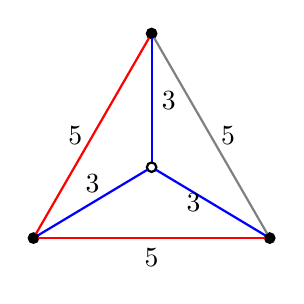
\begin{tikzpicture}
    [solid/.style={circle, draw=black,fill=black,thick,inner sep=0pt,minimum size=6mm,scale=0.2},
    empty/.style={circle, draw=black,thick,inner sep=0pt,minimum size=6mm,scale=0.2}]
    \node[solid] (a) at (-1.5,0) {};
    \node[solid] (b) at (1.5,0) {};
    \node[solid] (c) at (0,2.598) {};
    \node[empty] (o) at (0,0.9) {};

    \draw [red,thick] (a) -- (b) node[below,color=black,align=center,midway]{5};
    \draw [red,thick] (a) -- (c) node[left,color=black,align=center,midway]{5};
    \draw [black!50,thick] (b) -- (c) node[right,color=black,align=center,midway]{5};
    \draw [blue,thick] (a) -- (o) node[above,color=black,align=center,midway]{3};
    \draw [blue,thick] (b) -- (o) node[left,color=black,align=center,midway]{3};
    \draw [blue,thick] (c) -- (o) node[right,color=black,align=center,midway]{3};

\end{tikzpicture}
\caption{实心点集为$R$,$R$中的MST为红线;空心点集为$S$,蓝线组成Metric Steiner Tree。$MST=10<OPT=9$。}
\end{figure}

下面我们证明$R$中的最小生成树(MST)的解为最优解的2近似。

假设Metric Steiner Tree最优解为$G$,其权重之和为OPT。把最优解中的边都double 一下,我们得到了一个欧拉图$G'$(经过所有的边一次且仅一次,并回到出发点)。

%http://tex.stackexchange.com/questions/8652/what-does-t-and-ht-mean
\begin{figure}[!ht]
\centering
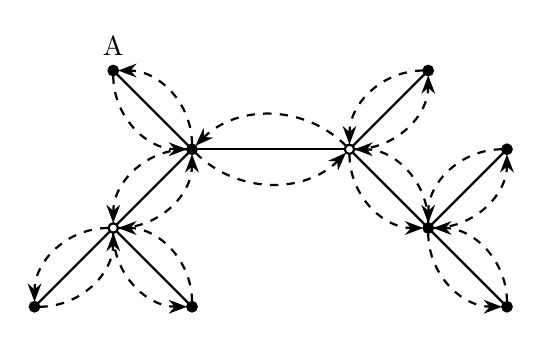
\begin{tikzpicture}
    [bend angle=45,
    solid/.style={circle, draw=black,fill=black,thick,inner sep=0pt,minimum size=6mm,scale=0.2},
    empty/.style={circle, draw=black,thick,inner sep=0pt,minimum size=6mm,scale=0.2}]
    \node[solid] (a) at (0,0) {};
    \node[solid] (b) at (2,0) {};
    \node[empty] (c) at (1,1) {};
    \node[solid] (d) at (2,2) {};
    \node[solid,label={A}] (e) at (1,3) {};
    \node[empty] (f) at (4,2) {};
    \node[solid] (g) at (5,3) {};
    \node[solid] (h) at (5,1) {};
    \node[solid] (i) at (6,2) {};
    \node[solid] (j) at (6,0) {};

    \draw [black,thick] (a) -- (c);
    \draw [black,thick] (b) -- (c);
    \draw [black,thick] (d) -- (c);
    \draw [black,thick] (d) -- (e);
    \draw [black,thick] (f) -- (d);
    \draw [black,thick] (f) -- (g);
    \draw [black,thick] (f) -- (h);
    \draw [black,thick] (h) -- (i);
    \draw [black,thick] (h) -- (j);

    \draw [-Stealth,dashed,black,thick] (a) to [bend right] (c);
    \draw [-Stealth,dashed,black,thick] (c) to [bend right] (b);
    \draw [-Stealth,dashed,black,thick] (b) to [bend right] (c);
    \draw [-Stealth,dashed,black,thick] (c) to [bend right] (d);
    \draw [-Stealth,dashed,black,thick] (d) to [bend right] (f);
    \draw [-Stealth,dashed,black,thick] (f) to [bend right] (h);
    \draw [-Stealth,dashed,black,thick] (h) to [bend right] (j);
    \draw [-Stealth,dashed,black,thick] (j) to [bend right] (h);
    \draw [-Stealth,dashed,black,thick] (h) to [bend right] (i);
    \draw [-Stealth,dashed,black,thick] (i) to [bend right] (h);
    \draw [-Stealth,dashed,black,thick] (h) to [bend right] (f);
    \draw [-Stealth,dashed,black,thick] (f) to [bend right] (g);
    \draw [-Stealth,dashed,black,thick] (g) to [bend right] (f);
    \draw [-Stealth,dashed,black,thick] (f) to [bend right] (d);
    \draw [-Stealth,dashed,black,thick] (d) to [bend right] (e);
    \draw [-Stealth,dashed,black,thick] (e) to [bend right] (d);
    \draw [-Stealth,dashed,black,thick] (d) to [bend right] (c);
    \draw [-Stealth,dashed,black,thick] (c) to [bend right] (a);
\end{tikzpicture}
\caption{实心点集为$R$,空心点集为$S$;实线为最优解$G$,其权重之和为OPT;虚线为边double之后的图$G'$,$G'$为一个欧拉图。}
\end{figure}

易知$G'$中的权重之和为2OPT。在$G'$中,从A点出发,逆时针遍历欧拉图,通过以下方法能得到$R$的一个Hamilton圈:删掉$R$和$S$之间的边,并越过$S$中的点,把$R$中的点连起来,并保证每个点只访问一次,由此得到$R$的一个Hamilton圈$G''$,如图Figure 3。

%http://tex.stackexchange.com/questions/8652/what-does-t-and-ht-mean
\begin{figure}[!ht]
\centering
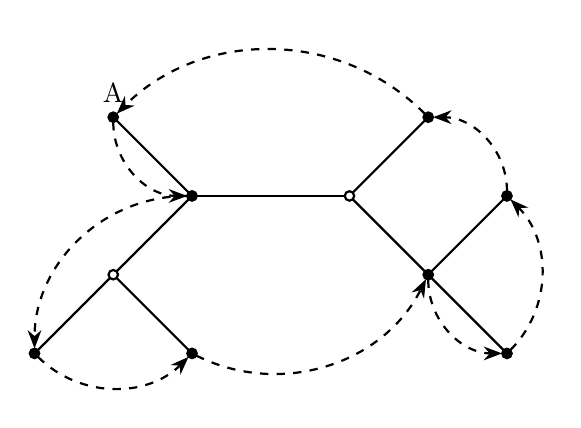
\begin{tikzpicture}
    [bend angle=45,
    solid/.style={circle, draw=black,fill=black,thick,inner sep=0pt,minimum size=6mm,scale=0.2},
    empty/.style={circle, draw=black,thick,inner sep=0pt,minimum size=6mm,scale=0.2}]
    \node[solid] (a) at (0,0) {};
    \node[solid] (b) at (2,0) {};
    \node[empty] (c) at (1,1) {};
    \node[solid] (d) at (2,2) {};
    \node[solid,label={A}] (e) at (1,3) {};
    \node[empty] (f) at (4,2) {};
    \node[solid] (g) at (5,3) {};
    \node[solid] (h) at (5,1) {};
    \node[solid] (i) at (6,2) {};
    \node[solid] (j) at (6,0) {};

    \draw [black,thick] (a) -- (c);
    \draw [black,thick] (b) -- (c);
    \draw [black,thick] (d) -- (c);
    \draw [black,thick] (d) -- (e);
    \draw [black,thick] (f) -- (d);
    \draw [black,thick] (f) -- (g);
    \draw [black,thick] (f) -- (h);
    \draw [black,thick] (h) -- (i);
    \draw [black,thick] (h) -- (j);

    \draw [-Stealth,dashed,black,thick] (a) to [bend right] (b);
    \draw [-Stealth,dashed,black,thick] (b) to [bend right] (h);
    \draw [-Stealth,dashed,black,thick] (h) to [bend right] (j);
    \draw [-Stealth,dashed,black,thick] (j) to [bend right] (i);
    \draw [-Stealth,dashed,black,thick] (i) to [bend right] (g);
    \draw [-Stealth,dashed,black,thick] (g) to [bend right] (e);
    \draw [-Stealth,dashed,black,thick] (e) to [bend right] (d);
    \draw [-Stealth,dashed,black,thick] (d) to [bend right] (a);
\end{tikzpicture}
\caption{实线为最优解$G$,虚线为用上述方法得到的只包含$R$中的点的Hamilton圈$G''$。}
\end{figure}

因为$G$有三角不等式的性质,所以$G''$中的权重和不超过$G'$中的权重和2OPT,如果删掉$G''$中的某条边,则得到$R$的一个生成树ST,ST的权重之和小于2OPT。又因为$R$中的最小生成树MST的权重之和小于ST的权重之和,所以MST<2OPT。

考虑图Figure 4的实例,外围的$n$个点组成集合$R$,集合$S$只包含中间一个点。$S$到$R$的边权重都为1,$R$之间的边权重为$2-\epsilon$,其中$\epsilon>0$是一个很小的数。$R$上的MST权重之和为$(n-1)(2-\epsilon)$,最优Metric Steiner Tree由中点到外围$n$个点及连边组成,$OPT=n$。$\lim\limits_{n\rightarrow \infty}\frac{MST(R)}{OPT}=\frac{(n-1)(2-\epsilon)}{n}=2$,说明2是不可改进的。

%http://tex.stackexchange.com/questions/8652/what-does-t-and-ht-mean
\begin{figure}[!ht]
\centering
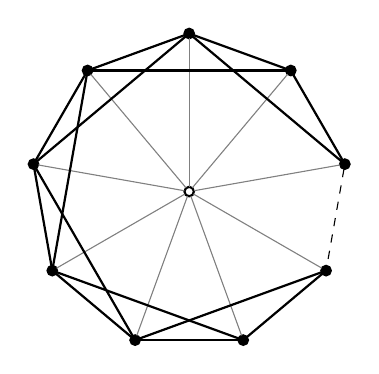
\begin{tikzpicture}
    [solid/.style={circle, draw=black,fill=black,thick,inner sep=0pt,minimum size=6mm,scale=0.2},
    empty/.style={circle, draw=black,thick,inner sep=0pt,minimum size=6mm,scale=0.2}]
    \node[draw=none,minimum size=4cm,regular polygon,regular polygon sides=9] (a) {};
    \node[empty] (0) at (a.center) {};
    % draw a black dot in each vertex
    \foreach \x in {1,2,...,9}
    {
        \node[solid] (\x) at (a.corner \x) {};
        \draw [black!50](0) -- (\x);
    }
    \foreach \x/\y/\z in {9/1/2,8/9/1,1/2/3,2/3/4,3/4/5,4/5/6,5/6/7}
    {
        \draw [black,thick](\x) -- (\y);
        \draw [black,thick](\x) -- (\z);
    }
    \draw [black,thick] (6) -- (7);
    \draw [dashed] (8) -- (7);
\end{tikzpicture}
\caption{外围的$n$个点组成集合$R$,集合$S$只包含中间一个点。$S$到$R$的边权重都为1,$R$之间的边权重为$2-\epsilon$,其中$\epsilon>0$是一个很小的数。}
\end{figure}

\section*{3\quad Vertex Cover}

给定图$G=(V,E)$,对图进行DFS,遍历过程中的非叶子节点构成集合$S$,则$S$是$G$的一个顶点覆盖,且$S$中顶点的数量小于最小顶点覆盖的2倍。

首先证明$S$是$G$的一个顶点覆盖。对于$G$中任意一条边$e_{ij}$,如果$i\in S$或$j\in S$,则$e_{ij}$被覆盖;如果$i\notin S$且$j\notin S$,说明$i,j$都是叶子节点,但是我们知道DFS过程中,叶子节点之间是不可能有边的,所以这样的$e_{ij}$不存在。$S$是$G$的一个顶点覆盖。

下面证明该算法是一个2近似的算法。

首先断言在最小顶点覆盖中不可能有叶子节点,因为叶子节点的父亲总是比叶子节点能覆盖更多的边,与其选叶子节点,不如选叶子节点的父亲。

对于任意一个顶点覆盖$VC$,因为$VC$至少要把所有边都覆盖住,所以有

\[
\begin{array}{c}
\sum_{v\in VC}deg(v)\geq |E| \tag{4}
\end{array}
\]

又因为一条边贡献了2度,所以

\[
\begin{array}{c}
\sum_{v\in VC}deg(v)+\sum_{v\notin VC}deg(v)=2|E| \tag{5}
\end{array}
\]

由(4)(5)得

\[
\begin{array}{c}
\sum_{v\notin VC}deg(v)\leq|E| \tag{6}
\end{array}
\]

由前面分析可知,不属于$VC$的点包括叶子节点$L$和非叶子节点中不是顶点覆盖的点$n-L-VC$,而非叶子节点的度数至少为2,所以有

\[
\begin{array}{crcl}
& |L|+2(n-|L|-VC) & \leq & |E| \tag{7} \\
\Leftrightarrow & 2n-|E|-|L| & \leq & 2VC \\
\Leftrightarrow & (n-|E|)+n-|L| & \leq & 2VC \\
\Rightarrow & 1+(n-|L|) & \leq & 2VC
\end{array}
\]

而$n-|L|$正是DFS中非叶子节点的个数,所以该算法是2近似的。
\section*{4\quad MAX-3SAT}
给定一个$3SAT$问题$\phi(x_1,...,x_n)=C_1\land...\land C_k$,对$n$个变量进行赋值,使得满足的子句越多越好。

本题介绍两种算法。
\subsection*{\textnormal{4.1\quad 1/2近似算法}}

\begin{codebox}
\Procname{$\proc{MAX-3SAT-APPROX1}(\phi)$}
\li \For $i$ = 1 \To $n$
    \Do
\li \If $x_i=true$ makes more clauses be true
    \Then
\li $x_i=true$
\li \Else
\li $x_i=false$
    \End
\li remove all true clauses from $\phi$
    \End
\li \Return $x$
\end{codebox}

对于每个变量$x_i$,尝试将其设为$true$或$false$,在所有包含$x_i$的子句中,如果$x_i=true$能让不少于一半的子句为$true$,则设置$x_i=true$,否则设置$x_i=false$;把为$true$的子句删掉,不断重复以上过程。

假设有$3SAT$:
\[
\begin{array}{c}
\phi(x_1,x_2,x_3)=(x_1\vee x_2 \vee \neg x_3)\land(\neg x_1\vee \neg x_2 \vee x_3)\land (\neg x_1 \vee x_2 \vee \neg x_3) \tag{8}
\end{array}
\]

对于$x_1$,设置为$true$只能保证第一个子句为$true$,而设置为$false$能保证后面两个子句为$true$,所以$x_1=false$。后续变量与此类似。

因为每次都至少使包含$x_i$的一半的子句为$true$,所以最终为$true$的子句数量至少为$k/2$,即该算法是1/2近似的。

\subsection*{\textnormal{4.2\quad 7/8近似算法}}

\begin{codebox}
\Procname{$\proc{MAX-3SAT-APPROX2}(\phi)$}
\li \For $i$ = 1 \To $n$
    \Do
\li Flip a fair coin
\li \If Heads
    \Then
\li $x_i=true$
\li \Else
\li $x_i=false$
    \End
    \End
\li \Return $x$
\end{codebox}

对每个变量以1/2的概率设置为$true$,以1/2的概率设置为$false$,则一个子句为$true$的概率为$(1-(\frac{1}{2})^3)=\frac{7}{8}$。定义随机变量:

\[
Z_j=
\begin{cases}
1 & \text{if clause $C_j$ is satisfied}\\
0 & \text{otherwise} \tag{9}
\end{cases}
\]

则$Z=\sum_{j=1}^kZ_j$就是为$true$的子句数量,其期望为:

\[
\begin{array}{c}
E[Z]=\sum_{j=1}^kE[Z_j]=\sum_{j=1}^kPr(C_j\text{ is satisfied})=\frac{7}{8}k\tag{10}
\end{array}
\]

所以该算法是一个7/8近似算法。
\end{document}
